\documentclass{tufte-book}

\usepackage[utf8]{inputenc} % uft8?
\usepackage[T1]{fontenc}

\usepackage{color}
\usepackage{xcolor}
\usepackage{framed}
\usepackage{listings}

\usepackage[normalem]{ulem}

\usepackage{multicol}              
\usepackage{multirow}
\usepackage{booktabs} 

\usepackage{mdframed}
\usepackage{mdwlist}

\usepackage{morefloats} % to take care of too many floats caused by the marginnotes

\usepackage[]{hyperref}
\definecolor{darkblue}{rgb}{0,0,.5}
\hypersetup{colorlinks=true, breaklinks=true, linkcolor=darkblue, menucolor=darkblue, urlcolor=darkblue, citecolor=darkblue}

\lstset{
language=[LaTeX]{TeX},
breaklines = true,
breakautoindent = false,
breakindent = 0pt,
commentstyle=\color{gray},
frame=single,
framerule=0.4pt,
framesep=3pt,
xleftmargin=3.4pt,
xrightmargin=3.4pt,
basicstyle=\normalfont,
keywordstyle=\color{blue}\sffamily,                                
identifierstyle=\color{black},
numbersep=5mm, 
numbers=left, 
numberstyle=\tiny,
morekeywords = {
maketitle, 
tableofcontents}  
}

\setcounter{secnumdepth}{1}


\title{Research skills\\
\large{An introduction to the crafts of a scientist}}
\author{Florian Hartig, University of Freiburg}

\begin{document}
\let\cleardoublepage\clearpage
\maketitle
\newpage
\tableofcontents

\newpage


\section*{Preface}

Lecture notes for the MSc course "Research Skills". Work in progress. Please send comments and suggestions to \href{http://florianhartig.wordpress.com/}{http://florianhartig.wordpress.com/}


\section*{Acknowledgments}

Severin Hauenstein for contributions to the chapter on scientific writing.

\chapter{Logic and philosophy of science}

\section{What is science?}

The Oxford dictionary defines science as 

\begin{quote}
Science [mass noun] - the intellectual and practical activity encompassing the systematic study of the structure and behaviour of the physical and natural world through observation and experiment
\end{quote}

Hence, science is a method to find out how to world works.\footnote{Epistemology, from Greek episteme = knowledge and logos = word is the branch of philosophy concerned with what knowledge is, how it can be acquired, and what can be known} In fact, "method" is an understatement. In the last centuries, the scientific method has been the reason for an unprecedented increase in knowledge, opportunity and well-being. In the western world at least, science is the current dominant answer to what one can know and how to find it out (epistemology). 

\marginnote{Many famous scientists engaged in personal feuds that, looking back, seem to be fueled by irrationality and personal pride. The doubtlessly ingenious Isaac Newton engaged in various spiteful and bitter feuds, including his most famous battle with German mathematician Gottfried Leibniz over the invention of infintesmial calculus.}

But science is also a human endeavor. If one says "science", it may be that the reference relates to the history of science, the state of scientific knowledge, or the science as a social institution. Regarding those latter aspects of science, things become less formally defined - if we look at the history of science, we see a complex of individuals that are somewhat unified by a common cause, but at the same time subject to their national and cultural influences as well as by personal vanity, pride or madness. As a result, the history of science, as well as its present state, is complicated by personal preferences, power games and random events, in the same way as political and economic history is.

In the center of science, though, is a set of assumptions and methods, a philosophy that allows us to draw and agree on conclusions from empirical observations. The rest of this chapter is devoted to understanding these assumptions somewhat better, and finding how how the "scientific method" works. 


\section{Philosophical foundations of scientific thinking}



\subsection{Rationalism}


In one of the foundational works of modern science, "Le Discours de la Méthode (1637)"  \footnote{The full title of this famous essay is "Discourse on the Method of Rightly Conducting One's Reason and of Seeking Truth" \citep{Descartes-DiscourseMethodRightly-1673}}, René Descartes famously observed: 

\begin{quote}
Good sense is, of all things among men, the most equally distributed; for every one thinks himself so abundantly provided with it, that those even who are the most difficult to satisfy in everything else, do not usually desire a larger measure of this quality than they already possess.
\end{quote}

These words of one of the founding fathers of what we today consider Science are often read and cited as a sarcastic observation of human vanity. However, if one continues reading, it becomes clear that Descartes may, after all, have been serious about his faith in human rationality. He goes on to state

\begin{quote}
And in this it is not likely that all are mistaken the conviction is rather to be held as testifying that the power of judging aright and of distinguishing truth from error, which is properly what is called good sense or reason, is by nature equal in all men; and that the diversity of our opinions, consequently, does not arise from some being endowed with a larger share of reason than others, but solely from this, that we conduct our thoughts along different ways, and do not fix our attention on the same objects. 
\end{quote}


\begin{figure}[]
\begin{center}
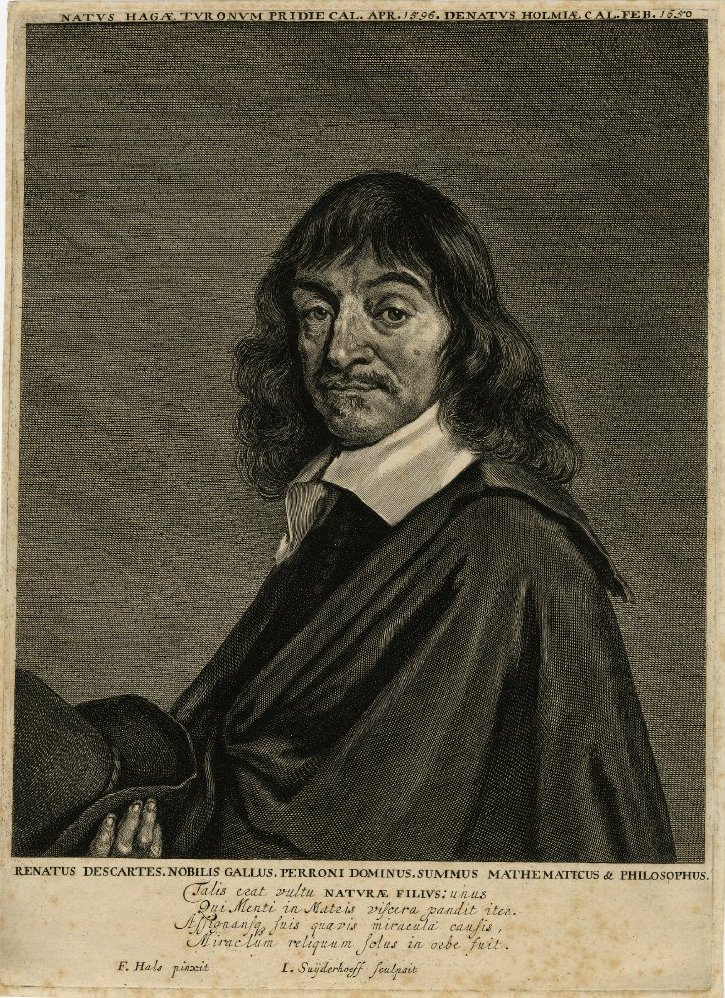
\includegraphics[width=5cm]{figures/Descartes}
\caption{Portrait of René Descartes}
\label{fig: Descartes}
\end{center}
\end{figure}



\subsection{Induction and deduction}

\subsection{Empiricism}


\section{Important philosophical views on science}


\subsection{Popper and the scientific method}


\subsection{Kuhn and variations of the scientific method}


\subsection{}


\section{Summary: the principles of science}





\chapter{The scientific literature}

Science today is highly specialized. Most basic questions have long been solved. You may think of the scientific enterprise as a "house of knowledge", where one story is built on the next. This is often expressed by a famous quote by Isaac Newton 

\begin{quote}
If I have seen further it is by standing on the shoulders of Giants.
\end{quote}

Regardless of whether the quote was meant as it is interpreted today \footnote{Brian Gottesman notes \href{http://mentalfloss.com/article/24520/6-things-you-should-know-about-isaac-newton}{here}: "Sir Isaac's most famous quotation may well have been an exercise in sarcastic, spiteful anger. In February 1676 Newton wrote to Hooke "if I have seen further it is by standing on the shoulders of Giants." Often taken as a sign of Newton's great humility, this famed quote was almost certainly intended as an insult to Hooke, who was hunchbacked and may have suffered from a form of dwarfism."
}, the fact remains that scientists today are hardly explorers that go far on unmarked territory. 


 

Before you start a new research project on a particular topic, you should find out what has already been done to a) understand better what you are doing b) avoid doing something that has already been done. 


\section{Finding relevant literature}

How to search for relevant literature depends on the


\section{Organizing your literature}

The basic answer to how to organize your literature is pleasingly short - people have created specialized software for this purpose. These reference managers work great, so use them! They will allow you to search in your papers for keywords, names, or anything else, link your pdfs, and they will also couple with your word processing software (MS Word, Open Office, LaTeX). 

\marginnote{See our lab on working with a reference manager \href{https://github.com/florianhartig/ResearchSkills/tree/master/Labs/LiteratureResearch}{here}}

The only question is which of the available programs work best for you. A general recommendation is difficult, as the choice depends next to your personal preferences also on you operating system and your word processing software. You'll find a lot of hints on the internet though, and I also give some short hints on the linked page to the right. 

\section{Citation rules}

\marginnote{High-profile cases of "faulty" citations include the former German Minister of Defense Karl-Theodor zu Guttenberg as well as the the former German Federal Minister of Education and Research, Annette Schavan}

Given the amount of PhD titles that have recently been revoked from prominent public figures for not correctly citing the literature in the PhD theses (a charitable expression for outright plagiarism in some cases)

http://www.nature.com/ng/journal/v47/n4/full/ng.3271.html

Greenberg-Howcitationdistortions-2009






\chapter{Questions, data and valid conclusions}

\begin{quote}
For to be possessed of a vigorous mind is not enough; the prime requisite is rightly to apply it. The greatest minds, as they are capable of the highest excellences, are open likewise to the greatest aberrations; and those who travel very slowly may yet make far greater progress, provided they keep always to the straight road, than those who, while they run, forsake it. (Descartes, Le Discours de la Méthode, 1637) 
\end{quote}


\section{What makes a good scientific questions?}

Assuming you have your question, how can we find an answer to this.



\section{Experimental design and validity}

\subsection{Constrcuct validity}

Are the things 

\subsection{Bias}


\citep{Ransohoff-Biasasthreat-2005}

\subsection{Internal validity}


\subsection{Statistical validity}


\paragraph{Statistical Power} Statististical power


\subsection{External validity}




\chapter{Principles and channels of communication}


\section{Principles of communication}



\section{Arguments and logical fallacies}


\section{Scientific visualisation}


\section{Communication channels}

\paragraph{Oral presentations}

\paragraph{Poster presentation}

\paragraph{Written texts}

\paragraph{Blogs, social media, and such}


\section{Hints on oral delivery}



Kelleher-Tenguidelineseffective-2011




\chapter{Scientific writing}


Writing is an essential skill for an academic, as for many other professions. \marginnote{The importance of the written word does not seem to change at all in the modern world. The art of writing, similar to public speaking, seems to be one of the stable skills that one can think of.} Despite its central role, however, few master it well. Writing is a subtle art. You can read some advice, but to become a skilled and effective writer requires a long process of observation, practice and reflection: read widely, and think about why some writers appeal to you more. Look critically over your own writing, and think about the things that you can improve. The rest of this section is intended to help you start this journey. 

\section{Some basic writing advice}

\paragraph{Start writing early}\marginnote{Please, follow this point in your thesis - if you don't it leads foreseeable into disaster!} Writing structures your thinking, and you will find flaws in your logic that you didn't see before. "The time to begin writing an article is when you have finished it to your satisfaction. By that time you begin to clearly and logically perceive what it is that you really want to say." (Mark Twain)

\paragraph{Know your audience}\marginnote{\citet{Gopen-ScienceOfScientific-1990} state "it matters only whether a large majority of the reading audience accurately perceives what the author had in mind".} Who is going to read what you write?  You need to adjust your text to the knowledge and background of your audience. 


\paragraph{Know what you want to say, and make a selection}\marginnote{"If you don't know where you are going,you'll end up someplace else" (Yogi Berra). } Sounds trivial, but in my experience it isn't. Before spending hours on writing the wrong text, try to explain a friend in 5-10 min the essential points of piece, and note the structure. If you fail with this, think again about your story. Also remember: Writing a good paper is not about telling everything you know or have done about a topic -- it is about telling a story and selecting the relevant details. 

\paragraph{Mindset} Make your goal, above all, clarity of thought and expression, and impervious logic of your argument. Read \citet{Woodford-Sounderthinkingthrough-1967}.

\paragraph{Respect conventions}\marginnote{For example, the default scientific article is divided into a title, abstract, introduction, materials and methods, results and discussion. Within these structural elements there are further recognizable patterns. Maintaining this structure makes it easier to understanding of the article's messages \citep{Gopen-ScienceOfScientific-1990,Tischler-Scientificwritingbooklet-1978}} Readers, particularly experienced readers, are familiar with writing conventions expect to find arguments, sections and statements in particular positions and structures. If the writer respects these structural standards the readability is greatly improved. 


\paragraph{Modesty} Think of a scientific text as a piece of craftsmanship, like a chair. What is expected of you is to produce a simple chair that respects the usual standards (e.g. four legs), and that is, above all, solid. You are not expected to add fancy ornamentation that might be used by an ingenious master craftsmen, and produce a entire set of furniture that would suffice to fit out a house. If you could do the later, you would gain admiration and praise, but when trying, you will nearly certainly fail to even produce the very thing you were asked for - a simple, solid chair. Bottomline: stay modest in what you want to achieve, but stay ambitions in how you achieve it!


\paragraph{Style} Writing is difficult. Good writing is incredibly hard. If you think writing is no problem for you, you probably haven't even realized the extent of your writing problems. Read the following section twice!


\section{Style}


\subsection{Sentence Structure}

\begin{quote}
The battle for good writing is won sentence by sentence! A good sentence is: short, has the subject and verb together, has an active verb, has the points of emphasis at the beginning and end, and moves the reader along from a familiar launch point at the start to the new information at the end. (Brian McGill, on the blog Dynamic Ecology)
\end{quote}



\subsection{Paragraph structure}

A paragraph is a logical unit of text. 

The first sentence provides the topic of the paragraph. The last sentence should, ideally, provide a closing 



\href{http://www.economist.com/styleguide/introduction}{http://www.economist.com/styleguide/introduction}

%\href{http://www.nature.com/authors/author_resources/how_write.html}{http://www.nature.com/authors/author_resources/how_write.html}



\subsection{Logic}


\subsection{Clarity}

Keep it simple. \footnote{Mark Twain is famous for his effective writing. A tip from him: "As to the Adjective: when in doubt, strike it out."}



\section{The structure of a scientific article}   
% general strucutre
On the largest unit of discourse the research paper comprises a title, abstract, keywords, and an introduction, methods, results and discussion section (and where required appendices). 
This structure somewhat forces the writer to repeat the story of the paper over and over again. In the end  it should be told roughly $3\frac{3}{4}$ times -- once with the title, once with the abstract, a quarter in the introduction, half in the discussion/ conclusion, and again once with the whole article.

%hourglass structure
Another structural element concerning the general layout is the "hourglass structure". This means the writer should start off with general information, becoming then more and more specific and completing with a link to the general again. Yet, it only applies to the abstract and (more flexibly) to the whole article.\\
 
%individual sections/elements
%title
\paragraph{Title}
Zooming in to the next smaller unit of discourse we start off with the title. %\marginnote{\large{\textsc{the title}}}
Its main purpose is to interest potential readers since 97~\%  of them only read the title. To keep them reading the title should signal the topic. A good tip is to make it precise and informative with a hint at the findings -- it should reflect the main message of the article's story.\\

%keywords
\paragraph{Keywords}
The author is asked to list some keywords, %\marginnote{\large{\textsc{the keywords}}}
which are usually located right below the abstract. These terms allow people to find the article when searching with ISI web of knowledge. Yet, since Google scans whole documents the keywords are probably not as important as they used to be. Nevertheless, a good strategy is to choose keywords complementary to title and abstract, e.g. for important technical terms that you
did not want to include in the abstract nor title.\\

%abstract
\paragraph{Abstract}
The abstract %\marginnote{\large{\textsc{the abstract}}} 
is the second time you will tell your story; in fact it can be considered as a mini paper. It starts off by setting the scene with a very short and general introduction. This usually links to the second part: Raise the problem. You can emphasize the research question by indicator words like "however". Here you tell why your work is necessary.\marginnote{To make sure you follow this structure it may be helpful to copy a template into your manuscript.} Third, you briefly delineate your approach. The fourth subsection serves to state the results. Finally, you present your conclusions and discuss the broader significance.\\

%introduction
\paragraph{Introduction}
The first main section of the article is the introduction. %\marginnote{\large{\textsc{the introduction}}}
It comprises four parts: Start of with one or two paragraphs outlining the broad topic and what work has been done before.\marginnote{Go from the general\\ ...to the specific\\ ...but not back to the general.} Here you usually cite a lot of literature showing that you know the current state of knowledge concerning the topic of your study.
Use another one or two paragraphs to explain the problem, i.e. the gap of knowledge. Here, you may sell your idea and why the knowledge gap needs to be filled.
Then, delineate your approach in one paragraph: What are your methods; what are the data you used?\marginnote{Make use of indicator words to clarify the role of the individual paragraph: however; problem/ challenge; here we used; we applied; we asked; we tested.}
Finally, you may list your specific research questions. This subsection does not need to be clearly separated from the approach subsection. It should however, provide a link to the result sections by outlining the work flow of the analysis.\\

%methods
\paragraph{Methods}
In the methods section %\marginnote{\large{\textsc{the methods}}}
the reader learns precisely what has been done. Even though details may be important this section should not take up too many words, since the total amount for the paper is usually fairly limited by the publishing journal\marginnote{Keyword is repdoucibility.}. You will have to make a selection here; technical information, which is necessary to replicate the study (Software version, etc.) can be moved to an (online) appendix. This may even increase the readability. If helpful the methods section may also be divided in subsections such as study area, data, statistical analysis/ model, analysis, etc. Another helpful tip is to add figures. They can greatly enhance the ability of the reader to understand your approach. Furthermore, if there were any problems with your methods, do not discuss them here -- use the discussion for that.\\

%results
\paragraph{Results}
Now that you have explained your methods and the course of analysis, present your results in the next section.%\marginnote{\large{\textsc{the results}}}
Here you will have to make a selection once again. The results you show need to be relevant to your story, and need to match the specific research questions you lay out in the abstract and more importantly at the end of the introduction. To clarify your findings it is helpful to use figures.\marginnote{Facts are better conveyed short and simple!}
Remember the most important aspect about this section: Your results need to be presented as neutral facts. Do only state what is obvious, but leave speculation for the discussion. You may however give an interpretation and cross links if they are obvious.\\

%discussion/conclusion
\paragraph{Discussion/ Conclusion}
Finally, we need to wrap up the article.%\marginnote{\large{\textsc{the discussion/ conclusions}}} 
The discussion/ conclusion section comes commonly at last but with extensive functionality. It contains a summary of the main findings. Remember here, many of your readers only read this section (and the title)\marginnote{Move from the specific\\ ...to the general.}. It is common to summarize by restating the problem, significance and the methods in the beginning. Secondly, this section is the platform to discuss the results, speculate about reasons and theories and for the connection to other literature.\marginnote{Only discuss the limitations that question/limit the credibility of your results.}
As was mentioned before, this section is the place where you may tell the reader about the limitations of your approach and possibly the reasons why the main findings are still credible. However, rather establish the domain under which your results are valid; do not question your approach in general. Finally, the reader expects you to provide conclusions, recommendations, applications and questions for further research.\\

\section{Showcase: A commented paper}

\begin{center}
	\huge{Fancy analysis supports hypothesis\marginnote{Try to capture the questions, methods, and main results of your study in the title, if possible} X as the main cause high species diversity in tropical forests} \\ 
	\vspace{0.3em}
	\large{Florian Hartig and Severin Hauenstein}\\
	\vspace{0.3em}
	\small{\textit{Department of Biometry and Environmental System Analysis, University of Freiburg, 79106 Freiburg, Germany}}\\
	\vspace{1em}
	\large{\today}\\
	\vspace{2em}
	\textbf{Abstract}\\ \marginnote{Remember: the abstract is a mini-paper}
\end{center}
\begin{quote}
Tropical forests are some of the most species-rich ecosystems\marginnote{First words set the scene} of the world.
The reason for this, \textbf{however}, is still widely debated\marginnote{Raise the problem. Indicator word: however}. Hypotheses range from processes related to productivity over environmental stability to the historical changes in geography.
\textbf{Here}\marginnote{Introduce your approach. Indicator word: here}, we contrasted these different hypotheses by using data from ... together with ... (fancy new method).
\textbf{We find that}\marginnote{State your results. Indicator word: We find, our results are ...} hypothesis X seems to be significantly better supported by our data
than all alternatives we tested. Specifically ... 
\textbf{In conclusion}\marginnote{Give your conclusions and discuss wider significance. Indicator word: in conclusion, ...}, our study supports the hypothesis that species diversity in the
tropics is mainly driven by higher productivity. These results challenge some long held
ideas about geographical stability being the main reason for global diversity
patterns. They also have important practical applications for mitigation of climate
change, as ...\\[0.3cm]
\noindent\textbf{Keywords:} Biodiversity -- Primary production -- Floristic structure ...\\
\end{quote}

\noindent\textbf{Introduction}\\
Tropical forests provide a suitable habitat to a vast variety of species. According to XY (19XX) tropical forests make up fo x \% of the planet's biodiversity.\\
...

Many ecologists have aimed at explaining this phenomena and a large number of hypotheses has been published in recent years (e.g. ABC, 19XX; D\&E, 20XX; FG, 20XX). However, not all of whom have made convincing arguments. To order the state of knowledge validation and comparison of the studies is desperately needed.\\
...

In this short note, we compare a set of pre-selected hypotheses published by ABC (19XX), D\&E (20XX), FG (20XX) and ... and present a validation of the used approaches. For the latter we used X data provided by XYZ (2014)\\
... 

We first test X in order to find the difference in Y. As an alternative approach we choose to look at Z for the purpose of XY. Specifically we are interested in species Y. Furthermore, the validation of the hypotheses will provide information about ...\\
...\\
In the following we briefly outline the concepts of ... and present our validation approach.\\
...

\noindent\textbf{Methods}\\

\noindent\textbf{Results}\\

\noindent\textbf{Discussion}\\
In this study, we used method X to test whether prevalence of A
is associated to factor B. Our main result is that there is a
significant correlation of B with A. This correlation, however, was
only found when factor C was also present.

Our findings support earlier findings of (X, 2005) and (Y, 2002)
who also found a positive correlation between A and B. The fact
that this correlation was only present in samples under conditions
C may also explain previous opposite results such as (ZZ,
2006,2008), as neither of these previous studies controlled for C.
The reason for this positive association and the fact that it is
affected by C is still unknown. We speculate that mechanism R
could be a reason for this. This idea is given further support by
the observation that the correlation between A and B is affected
by C. Such an effect would be expected if R is really the cause of
this Correlation, as R is dependent on C (XAY, 1968).



\section{A list of common writing problems}


\begin{enumerate}[(A)]


\item Strategic writing problems
\begin{enumerate}
	\item Do not make statements that are unnecessary for your argument, but could be questioned. 
	Example: "The two most classic games to simulate the behavior of animals are the Hawk-Dove game and the Prisoner's Dilemma." $\rightarrow$ Others might disagree. Is it really important to be so definite here? Why not say: "Two classic games..."?
	\item Passive/ Active: See the comments in the lecture notes on scientific writing. In general you should write in an active voice, unless  1) Sentence structure C3 takes precedence, or 2) the thing you talk about is impersonal, was done by another person. More details in the lecture notes. In particular, opinions of your own \textsc{should} be active.
	\item Be definite - remember Yoda: There is no try, do it. Phrases like: "we attempted to find whether there is" or "this study aims at" sound weak and defensive. Write "we studied whether ...". Also: "to the best of our knowledge ... " This is a borderline case. You will see this expression in scientific articles, and it's OK to use it. However, it does seem insecure. Better to indicate that you made some effort to find out together with such an expression. 	
	
 

\end{enumerate}

\item Logical problems
\begin{enumerate}
	\item The stated implication does not follow the argument logically. Example: "Because both models follow different pay-off schemes, it is important to know how a simulation model reacts to different settings." $\rightarrow$ Unclear why it is important to know how simulation reacts to different settings if two models are different.
	\item "Micrologic": Logical indicators such as "thus", "hence", "however", "nevertheless" have a clear and distinct meaning. "thus", "hence" indicate an implication. "however", "nevertheless" indicate contradicting statements or evidence to the previous proposition.
\end{enumerate}


\item Style
\begin{enumerate}
	\item Drop redundant words: Any of the following \textbf{words} can be erased: "\textbf{a total of} n subjects", "the simulations were run with the \textbf{exact} same parameter set as before"
	\item Pompous/ pontificating style: If something can be said in simple words, it should be said in simple words, i.e. if the only purpose of a sentence is to "sound scientific", it should not be said at all. Examples: The data \textbf{featured/comprised} a pixel size of 10 (had). We utilized (use).\footnote{Styleguides advice against complicated words such as utilize if there are simpler equivalent alternatives, although others have argued that there is a different between use and utilize - but could you name it? See discussion here \href{http://en.wiktionary.org/wiki/utilise}{here}.} We used the model in an integrated framework to facilitate a holistic forecast" (predicting from the model). Tip: Read \citet{Woodford-Sounderthinkingthrough-1967}.
	\item Topic position/ Stress position not properly occupied: The first part of a sentence should give the context. The last part of the sentence should provide the crucial new information, and should relate to what is further discussed. Tip: Read \citet{Gopen-ScienceOfScientific-1990}.
	\item A paragraph structures the text into topical units. Use them! Each paragraph should introduce its topic in the beginning, and ideally lead to some conclusion or summary at the end. 
	\item Unnecessary adjectives. Mark Twain: "As to the adjective: when in doubt, strike it out." Especially adjectives such as "very", "particularly" are often not necessary. Applies also to larger constructs such as "Evolutionary Game Theory \uline{is an important tool to} investigate(s) ..." -- if you erase the underlined text, the sentence remains fine.
	\item Unclear/ ambiguous expressions: Write as clear and as informative as possible. Avoid ambiguous words like "tends to", "mostly" etc. if you can make a definite statement. Example: "the frequency of cooperators always tends to be zero"  $\rightarrow$ What does that mean? 1) It was always zero or 2) It was zero in 95 \% of the cases or 3) something else.
\end{enumerate}

\item Grammar and spelling

\begin{enumerate}
	\item English commas have different rules than in German and other languages \url{http://www.grammarbook.com/punctuation/commas.asp}
	\item Wrong use of \textbf{which and that} Let's say that we have 10 samples. Compare the two sentences: 1) the samples, which were expose to radiation the day before, were analysed. 2) The samples that were exposed to radiation the day before were analyzed. The important difference is that 1) says all samples were exposed to radiation and then analysed, while 2) implies that not all samples were exposed to radiation, and only those that were were analysed. 1) is called a non-restrictive clause, and 2) is called a restrictive clause. "that" always implies a restrictive meaning. Additional confusion, however, is created by the fact that "which" can in fact be used for both, with a minor modification: if you want to use which restrictive, you have to write 3) The samples which were exposed to radiation the day before were analyzed. Notice that there is a tiny difference to 1) - there is no comma before which. This is the only indicator that allows us to know whether the restrictive or the non-restrictive meaning is implied. Many people are not aware of this difference though. In prose, the distinction may matter little, but for science, my opinion is that clarity goes before style, and I therefore recommend to strictly stay with 1) which for non-restrictive and 2) that for the restrictive meaning.
\end{enumerate}



\end{enumerate}


\section{Examples}

In the following, I highlighted \uline{redundant words} and other problems

\begin{itemize}

\item A \uline{subsequent} ANOVA \uline{analysis} \textbf{enabled a quantification of} the impacts of the varied factors (quantified)

\item There are \uline{a number of records} in the literature \uline{focusing on comparisons} between \uline{sets of }modeling approaches while predicting biomass at plot scale (A number of previous studies has compared modeling approaches to predict biomass at the plot scale)

\item \uline{As such}, the \uline{explicit} findings of our two experiments showed that \uline{a total of} 9 samples ... 

\end{itemize}


\chapter{A working scientists}

Up to now, we have covered the primary scientific process from deciding on a scientific question, generating valid data and conclusions, and communicating those in writing or through other channels. However, as hinted to in the introduction, science is also a human endeavor, and as such, a professional scientist should also be aware of the norms and codes of the field, as well as the realities of a life in science. The purpose of this chapter is to give a very fast overview on this questions.

\section{Professional ethics and good scientific practice}

The term "good scientific practice" encompass

\citep{Forschungsgemeinschaft-RulesGoodScientific-2013}

\marginnote{The rules of the German Science Foundation (DFG) are available \href{http://www.dfg.de/en/research_funding/principles_dfg_funding/good_scientific_practice/}{here}. Other guidelines for good scientific practice are available \href{https://github.com/florianhartig/ResearchSkills/blob/master/Labs/AcademicSoftSkills/codesOfConduct.md}{here}}


\subsection{Documentation}


There is no clear legal rule about how long data, documentation and samples have to be stored, but most funding organizations require 



\subsection{Honesty}




\marginnote{Simple things like having a good folder structure for each project help a lot. Have a look at our lab on \href{https://github.com/florianhartig/ResearchSkills/tree/master/Labs/ProjectOrganization}{project organization}}


\marginnote{When working with code, specially collaboratively, there is no way around using a version control system. See our lap on version control \href{https://github.com/florianhartig/ResearchSkills/tree/master/Labs/VersionControl}{here}}


\section{Social aspects}

\subsection{Collaborations and teams}

\subsection{Conflicts}

\subsection{Intercultural issues}


\section{Science as a career}



\marginnote{Read the special feature in Nature on the \href{http://www.nature.com/news/specials/phdfuture/index.html}{future of the PhD}}



\bibliographystyle{/Users/Florian/Home/Bibliography/Databases/bibstyles/elsart-harv-hyperlinks}
\bibliography{/Users/Florian/Home/Bibliography/Databases/flo}

\end{document}
